% vim: ts=4 sts=4 sw=4
\documentclass[portuguese, a4paper]{article}
\usepackage[T1]{fontenc}
\usepackage[utf8]{inputenc}
\usepackage{babel}
\usepackage[margin=2.5cm]{geometry}
\usepackage{lmodern}

\usepackage{graphicx}
\graphicspath{ {imagens/} }
\usepackage{wrapfig,lipsum}
\usepackage{bold-extra}
\usepackage{epstopdf}
\usepackage{float}
\usepackage{scalerel}
\usepackage{enumerate}
\usepackage{indentfirst}
\usepackage{mathtools}
\usepackage{amsmath}
\allowdisplaybreaks
\usepackage{amssymb}
\usepackage{listings}
\usepackage{color}
\usepackage{textcomp}
\usepackage{caption}
\usepackage{hyperref}
\hypersetup{
	colorlinks,
	citecolor=black,
	filecolor=black,
	linkcolor=black,
	urlcolor=blue
}

\newcommand\showdiv[1]{\overline{\smash{\hstretch{.5}{)}\mkern-3.2mu\hstretch{.5}{)}}#1}}
\newcommand\ph[1]{\textcolor{white}{#1}}
\newcommand\tu[0]{\textunderscore}

\definecolor{dkgreen}{rgb}{0,0.6,0}
\definecolor{gray}{rgb}{0.5,0.5,0.5}
\definecolor{mauve}{rgb}{0.58,0,0.82}
\definecolor{mygreen}{RGB}{28,172,0} % color values Red, Green, Blue
\definecolor{mylilas}{RGB}{170,55,241}

% ----- Cabeçalho e rodapé -----
\usepackage{fancyhdr}
\pagestyle{fancy}
\fancyhf{}

\renewcommand{\headrulewidth}{1pt}
\renewcommand{\footrulewidth}{0.5pt}

\rhead{2º Trabalho Computacional}
\lhead{Matemática Computacional}
\rfoot{Página \thepage}
\lfoot{\small Engenharia Eletrotécnica e de Computadores - IST}

\usepackage{pdfpages}

\begin{document}
\includepdf[pages={1}]{capa/capa.pdf}

% Secções em números romanos.
\renewcommand{\thesection}{\Roman{section}}

\tableofcontents
\newpage

\section{}
	\subsection{}
	\label{sec:I.1}
	\par
	Resposta no ficheiro \texttt{min\tu quad.m}, corrido pelo \emph{script} \texttt{1.m}, onde é possível alterar os pontos tabelados, os respetivos pesos e as funções de base.

	\subsection{}
	\par
	Para os dados tabelados:
	\begin{table}[H]
		\centering
		\begin{tabular}{c|c|c|c|c|c|c|c|c|c|c}
			\hline
			$1/e$	& 0.345	& 0.287	& 0.251	& 0.225	& 0.207	& 0.186	& 0.161	& 0.132	& 0.084	& 0.060	\\ \hline
			$s$		& 367	& 311	& 295	& 268	& 253	& 239	& 220	& 213	& 193	& 192	\\ \hline
			$d$		& 17	& 9		& 9		& 7		& 7		& 6		& 6		& 6		& 5		& 5		\\ \hline
		\end{tabular}
		\caption{Dados tabelados.}
	\end{table}

	\par
	Foram obtidas as três funções aproximadoras pedidas, através da função desenvolvida em \ref{sec:I.1}, pelos ficheiros \texttt{2\tu i.m}, \texttt{2\tu ii.m} e \texttt{2\tu iii.m}, corridos no \emph{script} \texttt{2.m}.

	\begin{figure}[H]
		\centering
		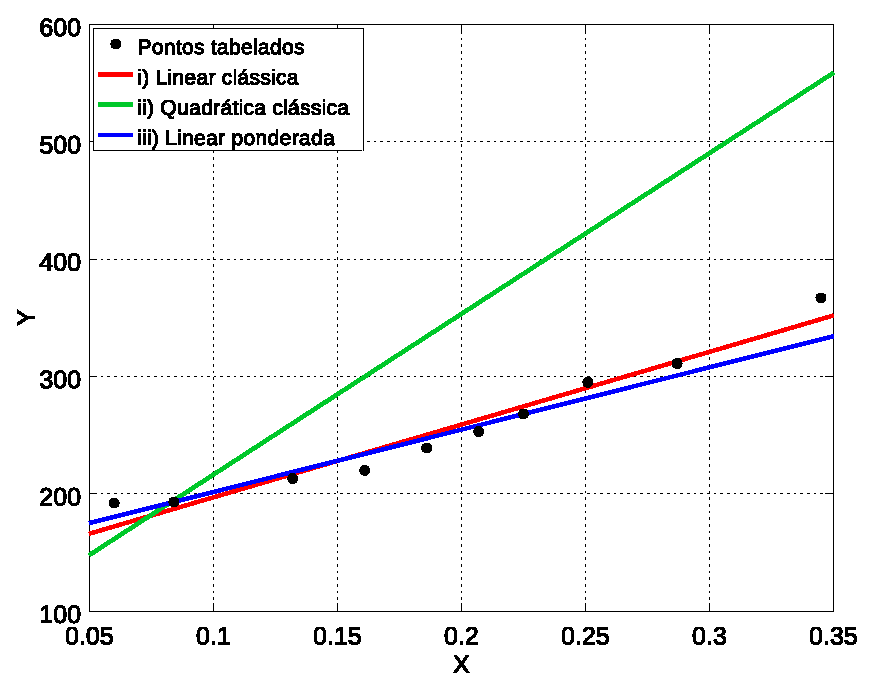
\includegraphics[width=0.80\linewidth]{l}
		\captionsetup{width=0.80\linewidth}
		\caption{Diferentes funções aproximadoras dos pontos tabelados pelo critério dos mínimos quadrados clássico e ponderado.}
	\end{figure}


\section{}
	subsection{}
	\par


\end{document}
